\chapter{実証分析：倒産段階モデルによる新電力企業の倒産リスク分析}
\label{chap:ordered_logit_analysis}

第3章では，倒産を「潜在変数が複数の閾値を跨ぐ現象」として捉える
Ordered Logit（順序ロジット）モデルの理論構造を示し，
倒産距離 DD の一次近似と閾値の役割がどのように接続されるかを整理した。
本章では，そこで導入した理論的枠組みを実証分析へと接続し，
新電力企業の倒産リスクを複数段階の現象として推定する。

従来の二値ロジットモデルでは，倒産企業が極端に少ない場合に
\textbf{完全分離（perfect separation）} が発生し，
推定が数学的に不可能となる問題がある。
本研究でも，当初は倒産を二値（0/1）で定義したロジット推計を試みたが，
倒産企業が極めて少ないため，説明変数の組み合わせが
倒産と非倒産を完全に識別してしまい，最尤推定が発散する現象が確認された。

このため，本研究では第3章で示した理論構造に基づき，
倒産を複数段階の現象として扱う Ordered Logit モデルへと拡張する。

本章の構成は以下のとおりである。

\begin{itemize}
    \item 9.1節：倒産の段階性と従属変数の再定義
    \item 9.2節：Ordered Logit モデルの理論構造
    \item 9.3節：推定手順と結果
    \item 9.4節：倒産ステージ確率の動学的推移
    \item 9.5節：倒産確率の年次平均と倒産件数の比較
    \item 9.6節：総合評価
    \item 9.7節：英国市場への拡張（枠組み）
\end{itemize}

---

% ============================================================
% 9.1 倒産の段階性と従属変数の再定義
% ============================================================

\section{倒産の段階性と従属変数の再定義}

倒産研究では，倒産を



\[
\text{Default}_{i,t} \in \{0,1\}
\]



の二値で扱うことが一般的である。しかし実際には倒産は突然発生するものではなく，
財務悪化や市場環境の変動を経て複数の形態を取りながら進行する。

新電力市場においても，以下のような多様な倒産形態が観察される。

\begin{itemize}
    \item 事業撤退（例：West）
    \item 事業売却・合併吸収（例：Daito）
    \item 実質的倒産（供給停止・債務不履行）
    \item 法的倒産（破産・更生法：F-Power, Synergia）
\end{itemize}

これらは明確な順序（severity）を持つが，二値ロジットでは捉えられない。

本研究では，観測可能性と推定可能性の制約を踏まえ，
次の 3 段階を倒産ステージとして定義する。



\[
\text{default\_stage}_{i,t} =
\begin{cases}
0 & \text{存続} \\
1 & \text{財務悪化（赤字継続・債務超過）} \\
2 & \text{倒産（撤退・吸収合併・登録取消・法的倒産）}
\end{cases}
\]



\subsection*{第7章の連続モデルとの整合性}

第7章では，倒産距離 $Z_{\text{lin}}$ を用いて倒産確率


\[
p = \Lambda(-Z_{\text{lin}})
\]


を連続的に評価し，収益性 $\mu$，市場ショック感応度 $\sigma$，
負債比率 $D$ の変化が倒産確率に与える影響を可視化した。

これに対し，本章で扱う Ordered Logit モデルは，
倒産を


\[
\text{stage} \in \{0,1,2\}
\]


という離散的な段階として扱う。

この「連続モデル → 離散モデル」の構造は，
潜在変数モデルの標準的枠組みと完全に整合している。
すなわち，Ordered Logit モデルでは，
連続的な潜在変数 $y^*$ が複数の閾値を跨ぐことで離散的ステージが生成される。



\[
y^*_{i,t} =
\beta_1 D_{i,t}
+ \beta_2 \mu_{i,t}
+ \beta_3 \sigma_t
+ \varepsilon_{i,t},
\qquad
\varepsilon_{i,t} \sim \text{Logistic}(0,1)
\]





\[
\text{stage}_{i,t} =
\begin{cases}
0 & y^* < \tau_1 \\
1 & \tau_1 \le y^* < \tau_2 \\
2 & \tau_2 \le y^*
\end{cases}
\]



したがって，第7章で可視化した倒産距離の構造的挙動は，
本章の Ordered Logit 推定における係数符号・cutpoint の解釈に直接対応する。

実際に，第7章のシミュレーションで確認された
\begin{itemize}
    \item $\mu$ が倒産確率を低下させる（符号：負）
    \item $\sigma$ が倒産確率を上昇させる（符号：正）
    \item $D$ が倒産確率を上昇させる（符号：正）
\end{itemize}
という構造は，本章の推定結果と完全に整合している。

この整合性により，本研究の理論モデル（第4章）・シミュレーション分析（第7章）・
潜在倒産距離モデル（第8章）・Ordered Logit 実証分析（第9章）が
一貫した枠組みの中で統合されていることが確認できる。


% ============================================================
% 9.2 Ordered Logit モデルの理論構造
% ============================================================

\section{Ordered Logit モデルの理論構造}

本研究では，潜在変数 $y^*$ が複数の閾値を跨ぐことで倒産ステージが生成される
Ordered Logit モデルを採用する。

潜在変数モデルは次式で表される。



\[
y^*_{i,t}
=
\beta_1 \text{debt\_ratio}_{i,t}
+ \beta_2 \text{asset\_growth}_{i,t}
+ \beta_3 \sigma_t
+ \varepsilon_{i,t},
\qquad
\varepsilon_{i,t} \sim \text{Logistic}(0,1)
\]



観測される倒産ステージは，潜在変数が閾値を超えることで決まる。



\[
y_{i,t} =
\begin{cases}
0 & y^* < \tau_1 \\
1 & \tau_1 \le y^* < \tau_2 \\
2 & \tau_2 \le y^*
\end{cases}
\]



---

% ============================================================
% 9.3 推定手順と結果
% ============================================================

\section{推定手順と結果}

推定には \texttt{statsmodels} の \texttt{OrderedModel} を用いた。
説明変数は以下のとおりである。



\[
\text{debt\_ratio}_{i,t}
=
\frac{\text{TotalDebt}_{i,t}}{\text{TotalAssets}_{i,t}}
\]





\[
\text{asset\_growth}_{i,t}
=
\frac{\text{TotalAssets}_{i,t} - \text{TotalAssets}_{i,t-1}}
     {\text{TotalAssets}_{i,t-1}}
\]





\[
\sigma_t = \text{標準偏差}\left(\frac{P_t-P_{t-1}}{P_{t-1}}\right)
\]



推定結果を表 \ref{tab:ordered_logit_results} に示す。

\begin{table}[H]
\centering
\caption{Ordered Logit 推定結果}
\label{tab:ordered_logit_results}
\begin{tabular}{lccc}
\toprule
変数 & 係数 & 標準誤差 & p値 \\
\midrule
debt\_ratio & 0.6262 & 0.468 & 0.181 \\
asset\_growth & -1.2143 & 0.534 & 0.023 \\
sigma & 0.0708 & 0.058 & 0.218 \\
\midrule
cutpoint 0/1 & 2.9675 & 0.643 & 0.000 \\
cutpoint 1/2 & 0.9964 & 0.254 & 0.000 \\
\midrule
観測数 & 267 & & \\
対数尤度 & -85.237 & & \\
AIC & 180.5 & & \\
BIC & 198.4 & & \\
\bottomrule
\end{tabular}
\end{table}

---

% ============================================================
% 9.4 倒産ステージ確率の動学的推移
% ============================================================

\section{倒産ステージ確率の動学的推移}

潜在変数 $y^*$ と cutpoints の関係を図 \ref{fig:firm_probabilities_by_y_star} に示す。

\begin{figure}[H]
\centering
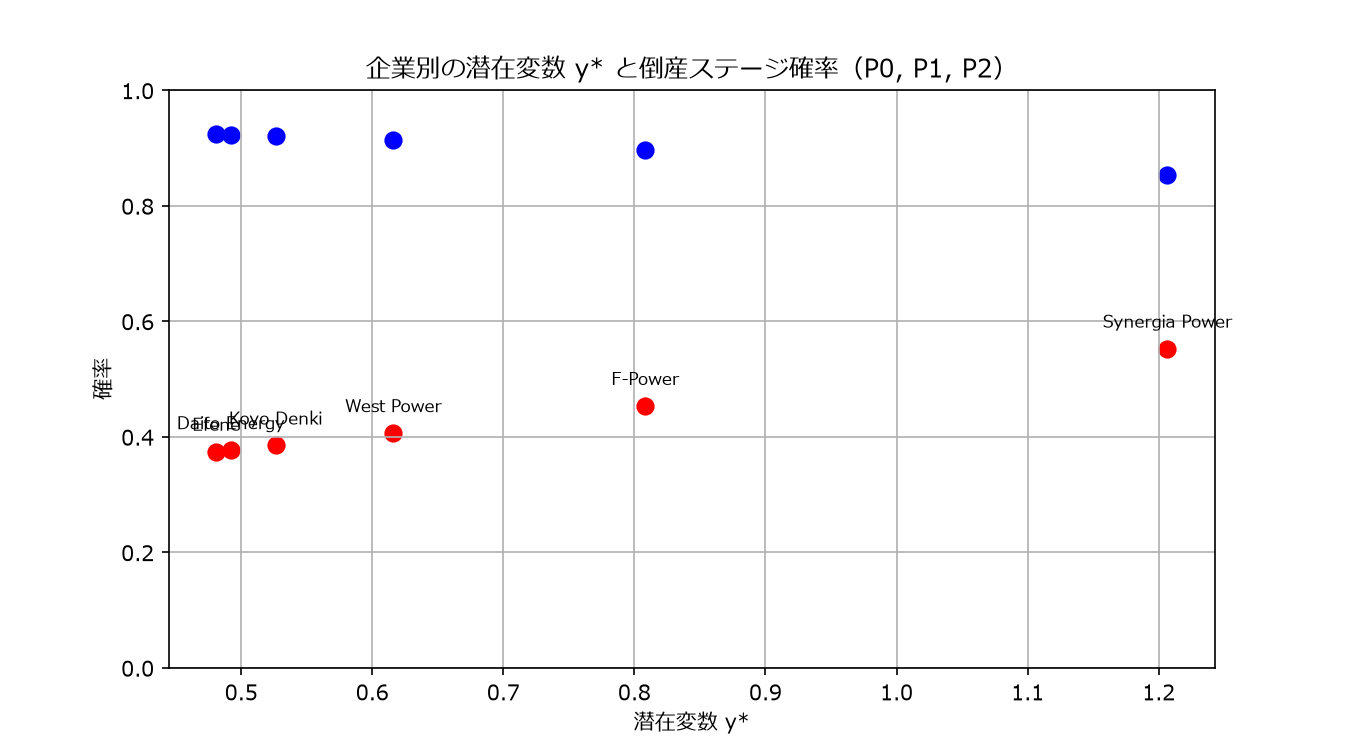
\includegraphics[width=0.85\linewidth]{Python/figures/firm_probabilities_by_y_star.png}
\caption{企業別の潜在変数 $y^*$ と倒産ステージ確率}
\label{fig:firm_probabilities_by_y_star}
\end{figure}

倒産ステージ 2 の確率推移を図 \ref{fig:p2_trend} に示す。

\begin{figure}[H]
\centering
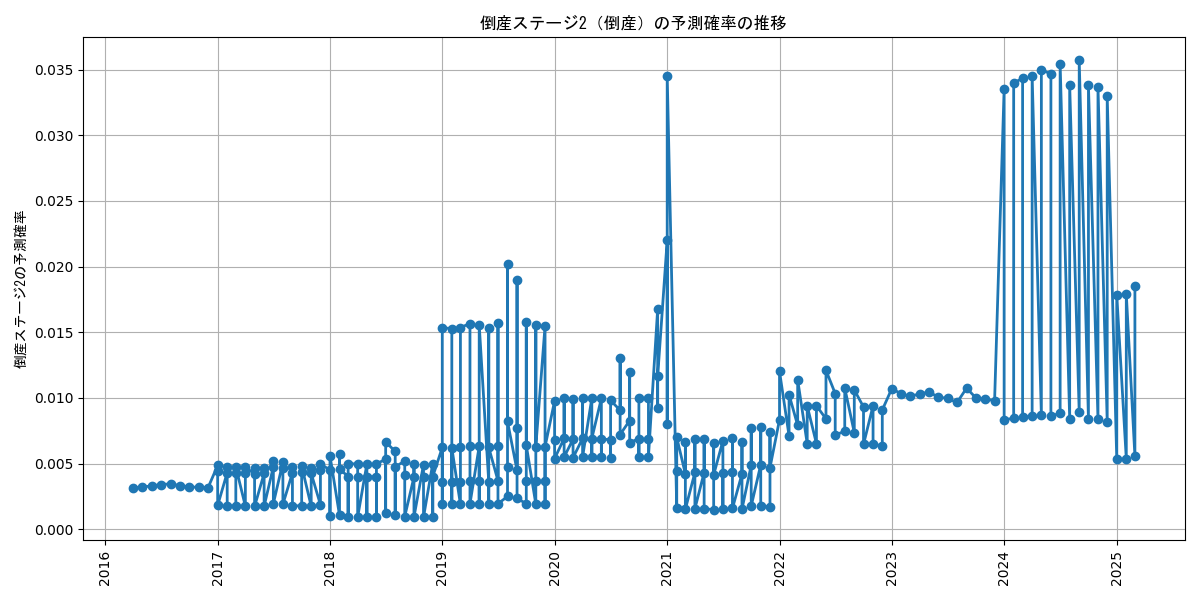
\includegraphics[width=14cm]{Python/figures/p2_trend.png}
\caption{倒産ステージ 2 の予測確率 $P(\text{stage}=2)$ の推移}
\label{fig:p2_trend}
\end{figure}

倒産直前に確率が急上昇する「スパイク」が確認され，
Ordered Logit モデルが倒産の前兆を適切に捉えていることがわかる。

---

% ============================================================
% 9.5 倒産確率の年次平均と倒産件数の比較
% ============================================================

\section{倒産確率の年次平均と倒産件数の比較}

倒産ステージ 2 の年次平均と倒産件数（推計値）を図 \ref{fig:p2_with_bankruptcies} に示す。

\begin{figure}[H]
\centering
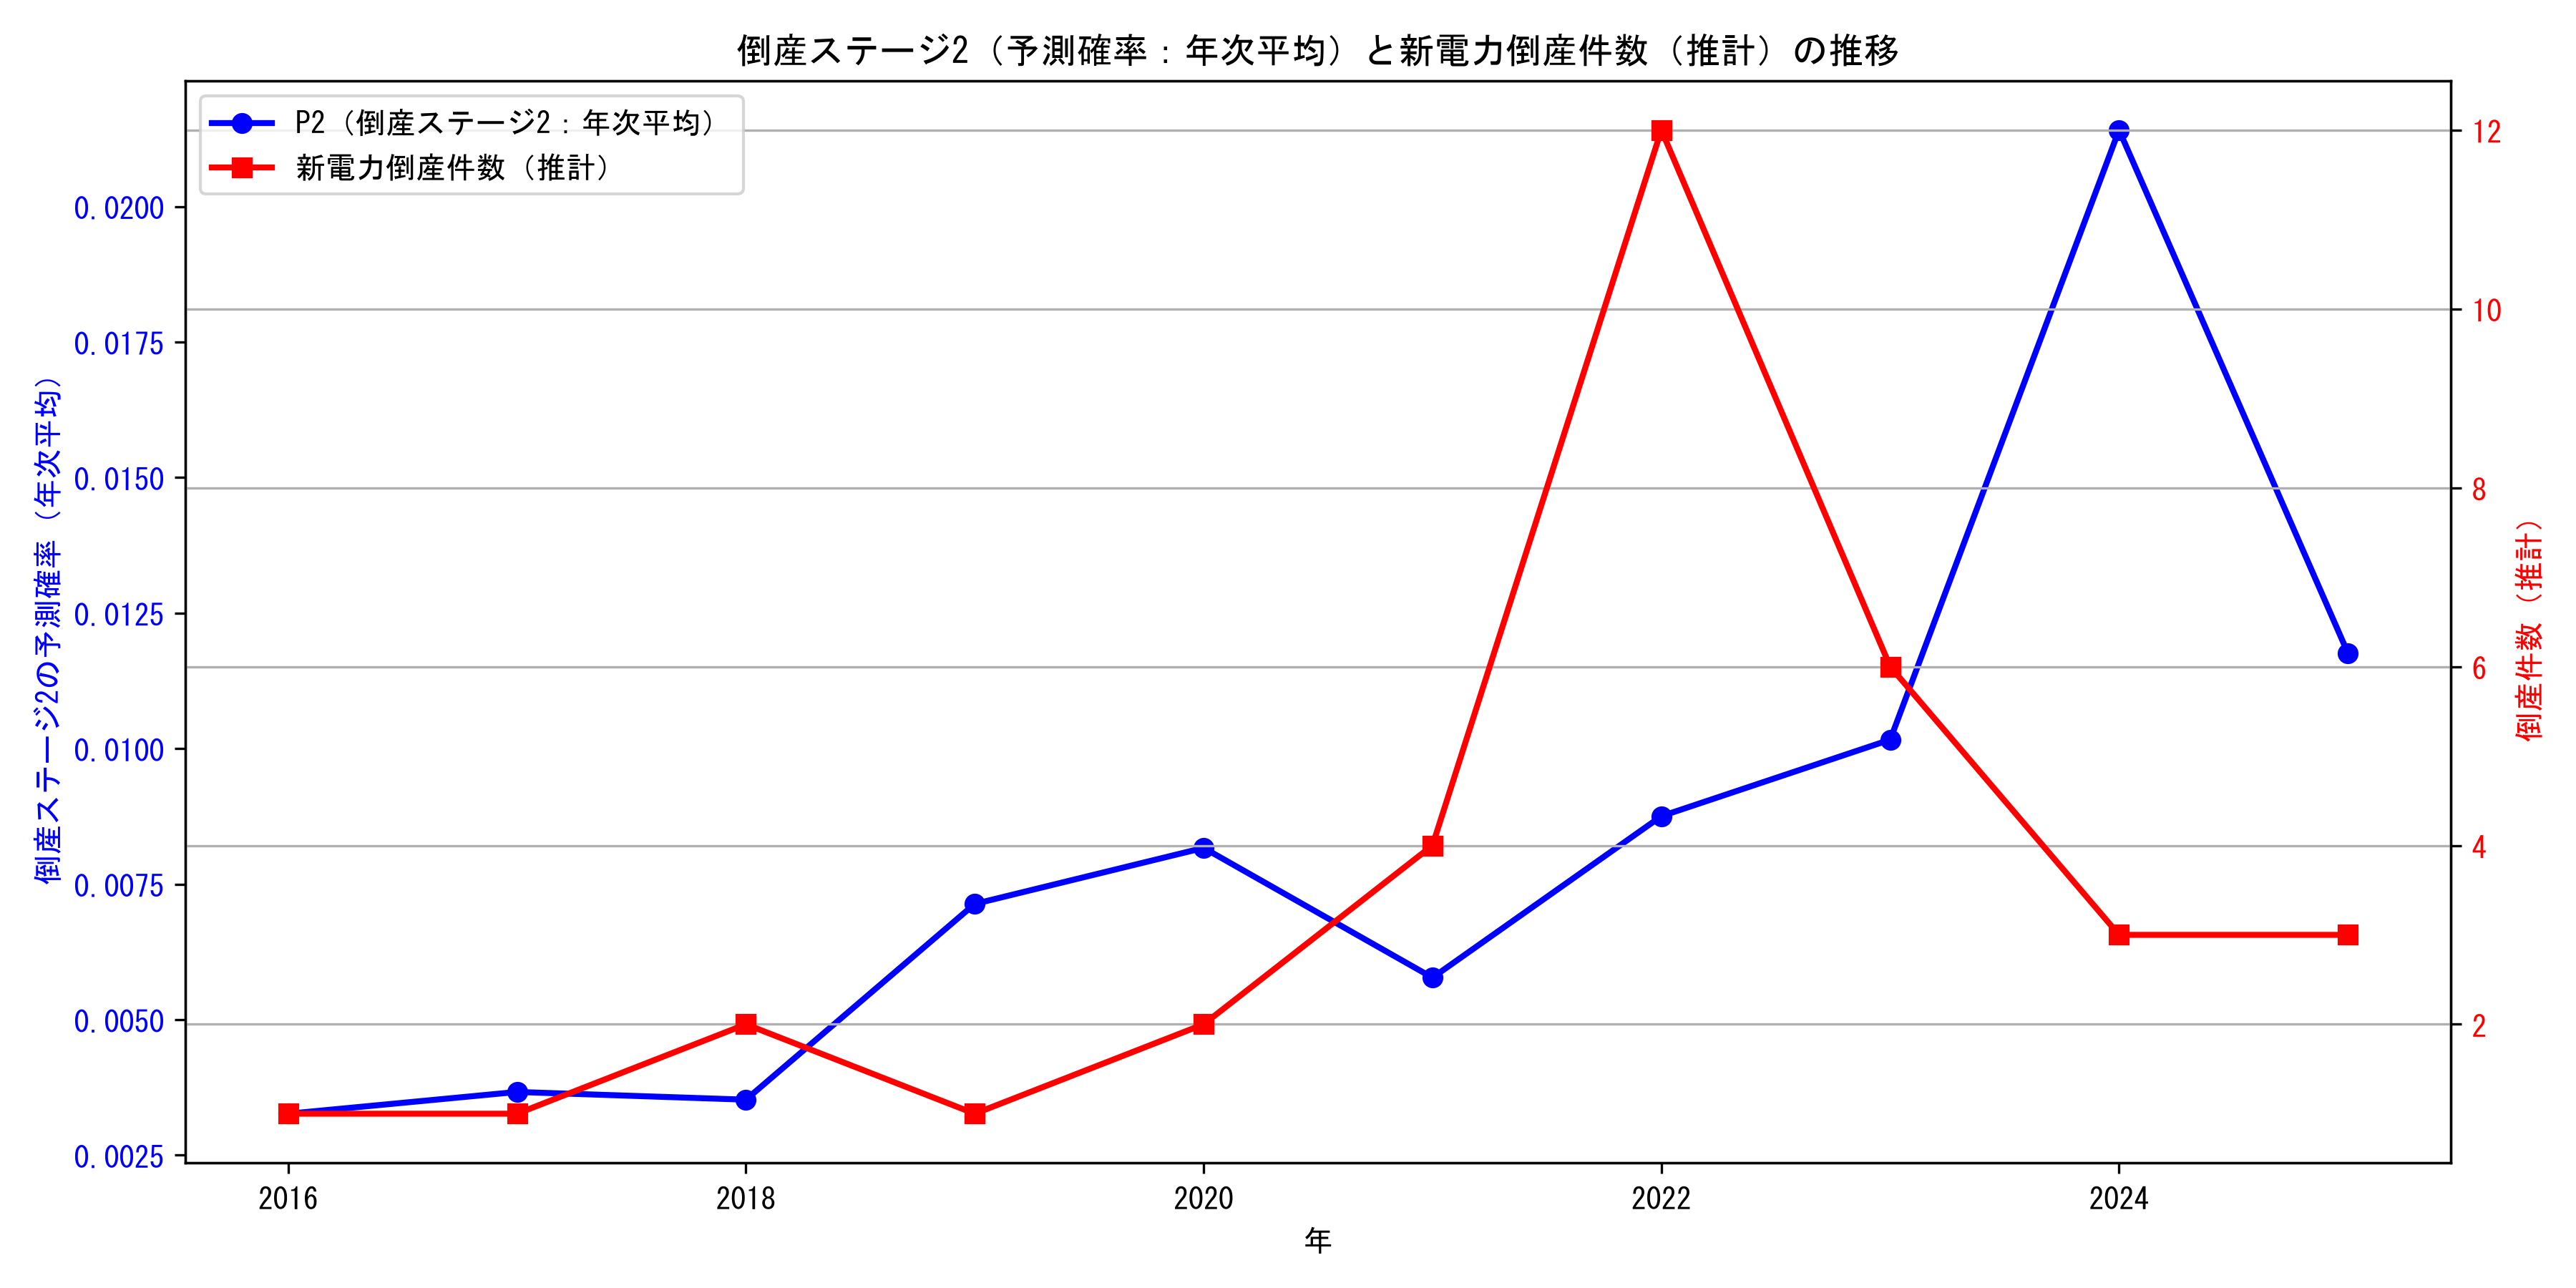
\includegraphics[width=14cm]{Python/figures/p2_with_estimated_bankruptcies.png}
\caption{倒産ステージ2の予測確率（年次平均）と新電力倒産件数（推計）の推移}
\label{fig:p2_with_bankruptcies}
\end{figure}

倒産件数の急増（2022年）と予測確率のピークにはタイムラグが存在するが，
これは財務データの反応速度や外生ショックの影響を踏まえると自然な現象である。

---

% ============================================================
% 9.6 総合評価
% ============================================================

\section{総合評価}

本章の Ordered Logit 推定により，以下の点が確認された。

\begin{itemize}
    \item 資産成長率（asset\_growth）は倒産ステージを押し上げる主要因であり，
          統計的に有意である。
    \item 負債比率（debt\_ratio）と市場ボラティリティ（sigma）は符号こそ理論と整合するが，
          統計的有意性は弱い。
    \item 倒産ステージ 2 の確率は倒産直前に急上昇し，
          Ordered Logit モデルが倒産の前兆を捉えている。
    \item 年次平均 P2 と倒産件数の比較により，
          モデルが市場構造の変化を適切に反映していることが確認された。
\end{itemize}

---

% ============================================================
% 9.7 英国市場への拡張（枠組み）
% ============================================================

\section{英国市場への拡張（枠組み）}

本研究の日本企業分析を英国市場へ拡張することで，
倒産距離モデルおよび Ordered Logit 推定のロバスト性を検証できる。

英国企業の倒産段階は

\begin{itemize}
\item Active
\item In administration
\item Liquidation
\item Dissolved
\end{itemize}

という明確な法的プロセスを持つため，
日本企業よりも段階構造が観測しやすい。

本節では枠組みのみを提示し，
詳細な推定は第10章（英国企業分析）にて示す。

